\subsection{Tekstlig Use Case}
\begin{table}[H]
\centering
\label{tab:tuc4}
\begin{tabular}{| l | L{4in} |}
\hline
Use Case & Scenario 3 \\
\hline
Aktør & Møteleder og inviterte ansatte \\
\hline
Trigger & Møtelederen avlyser møtet \\
\hline
Pre-betingelser & Møtelederen har laget møtet og invitert andre ansatt. Noen ansatt må også ha godtat møtet. \\
\hline
Post-betingelser & Møten slettes og det gis bedskjed til de involverte ansatt. \\
\hline
Normal hendelsesflyt & 
\begin{minipage}{4in}
\vskip 4pt
\begin{itemize}
\item Møtelederen avlyser møtet.
\item Møtet blir slettet fra Møtelederens personlige kalender.
\item En melding blir sendt til alle inviterte medlemer.
\end{itemize}
\vskip 4pt
\end{minipage}
 \\
\hline
Variasjoner & \\
\hline
Relatert informasjon & De inviterte medlemer ser meldingen neste gang de logger seg på systemet. \\
\hline
\end{tabular}
\caption{Tekslig Use Case-diagrame}
\end{table}

\subsection{Sekvensdiagram}
\begin{figure}[H]
\label{fig:sek4}
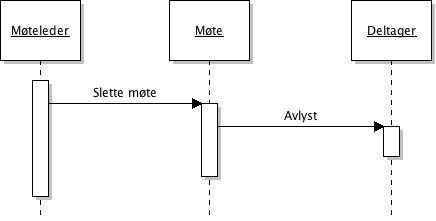
\includegraphics[width=400px]{sekvens4.png}
\caption{Use Case-diagram for scenario 4}
\end{figure}